\input{text/diss}

\begin{document}

\def\labauthors{Войтович Д.А., Понур К.А.}
\def\labgroup{440}
\def\labnumber{2}
\def\labtheme{Исследование биполярных процессов переноса тока в тлеющем разряде}
\renewcommand{\vec}{\mathbf}
\renewcommand{\phi}{\varphi}
\renewcommand{\hat}{\widehat}

\input{text/titlepage}

\section{Теоретическая часть}
\subsection{Основные части тлеющего разряда}
Через разрядный промежуток электроны проходят значительно быстрее ионов. Значит, в разрядном промежутке, как только
 создается условие для ионизации газа электронами, начинает накапливаться положительный пространственный заряд 
 ионов.

Рассмотрим, как будет меняться распределение потенциала между электродами (рис.1). Прямая 1 - распределение
 потенциала в начале разряда. Выделим группу электронов начинающих двигаться от катода и набирающих скорость,
 достаточную для ионизации вблизи анода. После их прохождения вблизи анода останутся малоподвижные плюс-тоны и
  кривая распределения потенциала примет вид 2. Поле вблизи катода станет больше. Вторая партия, состоящая из 
  электронов, образованных на пути следования первой партии, и фотоэлектронов из катода, создает пространственный 
  заряд вблизи $A_2$ и кривая потенциала примет вид 3. Расчет показывает, что после прохождения 3-4 электронных 
  лавин, кривая рапределения потенциала 4 стабилизируется и будет показывать резкое падение потенциала вблизи 
  катода (катодное падение) вследствие образования положительного пространственного заряда, что произойдет очень 
  быстро из-за малого времени пробега электронов.

  Разделение электронов на партии - искусственный прием. В действительности, изменение формы кривой потенциала 
  происходит непрерывно. Разряд, характерной особенностью которого является большое катодное падение потенциала -
   тлеющий разряд, обычно устанавливается при небольших давлениях. Катодные части разряда занимают всего несколько 
   миллиметров вблизи катода. Можно считать, что размер области катодного падения равен 10-12 свободным пробегам 
   электрона, на таком пути практически все электроны испытывают хотя бы одно соударение. Чем меньше давление, тем 
   длиннее область катодного падения.

  \begin{figure}[h!]
	\centering
	\includegraphics[width=0.5\linewidth]{fig/img1.jpg}
	\caption{Установление распределения потенциала в тлеющем разряде}
	\label{fig:1}
\end{figure}

Механизм поддержания разряда можно представить себе в таком виде: электроны, освобожденные из катода в результате 
$\gamma$-процессов, набирают сначала скорость и, пройдя некоторый путь, приобретают энергию, достаточную для 
ионизации и при том такую, при которой вероятность ионизации близка к максимуму (при соударении вероятность ионизации 
быстрыми электронами мала, а медленные электроны, энергия которых меньше энергии ионизации, совсем не могут 
ионизировать газ). В результате появляется область, где происходит много ионизаций, т.е. накапливается большой
положительный пространственный заряд - это и есть область катодного падения.

Следующая область тлеющего разряда - положительный столб, который представляет собой высокоионизированный и 
электрически квазинейтральный газ, называемый плазмой. Большая концентрация заряженных частиц обуславливает 
высокую проводимость плазмы. Свечение плазмы - это свечение атомов, переходящих из возбужденного состояния в нейтральное.
Большая часть заряженных частиц производится в ней самой при ионизирующих столкновениях. Только небольшая часть 
электронов входит в плазму из других частей разряда. Чтобы плазма могла существовать и чтобы число вновь создавшихся 
ионов равнялось числу исчезнувших, в газоразрядной плазме должен существовать продольный градиент потенциала. В 
стационарном состоянии оба этих процесса генерации и рекомбинации ионов вполне скомпенсированы. В тлеющем разряде 
положительный столб играет роль провода, соединяющего прикатодные части разряда с анодом, ничего не прибавляя к катодной
части разряда и ничего не отнимая от нее.

\subsection{Вольт-амперная характеристика тлеющего разряда}
Если к электродам разрядной трубки приложено напряжение, достаточное для зажигания разряда, то в зависимости от 
давления газа, мощности источника напряжения и внешнего сопротивления, включенного в цепь трубки, установится тихий,
тлеющий или дуговой разряд. При этом конечная форма будет развиваться из так называемого "тихого разряда", который 
характеризуется малой плотностью тока и незначительным пространственным зарядом. Переходные формы разряда можно 
стабилизировать путем введения последовательно с трубкой большого омического сопротивления.

Пр  постепенном уменьшении этого сопротивления сила тока через трубку будет возрастать при одновременном изменении 
напряжения на клеммах трубки. Зависимость напряжения от силы тока в этом случае изображается кривой ABCDE (рис.2). 
Для удобства на оси абсцисс откладывается $ln J$. Отрезок АВ соответствует несамостоятельному разряду, BC - переходной 
стадии разряда, CDE - тлеющему разряду. Таким образом, вольт-амперная характеристика тлеющего разряда состоит из 
двух ветвей, из которых одна - падающая - разряд с нормальным катодным падением, другая - возрастающая - разряд с 
аномальным катодным падением.

\begin{figure}[h!]
	\centering
	\includegraphics[width=0.5\linewidth]{fig/img2.jpg}
	\caption{Вольт-амперная характеристика тлеющего разряда}
	\label{fig:2}
\end{figure}

На участке CD разряд находится в стадии нормального тлеющего разряда. Это значит, что катодное падение должно оставаться 
величиной постоянной (здесь справедлив закон Геля). Но падение потенциала складывается из катодного падения и падения 
потенциала на положительном столбе, которое уменьшается с возрастанием тока. Следовательно, и вся разность потенциалов 
между электродами будет уменьшаться с увеличением силы тока. На участке DE разряд уже будет аномальным и, следовательно,
 катодное падение в этом случае увеличивается с увеличением силы тока и при том в большей степени, чем уменьшается 
 градиент в положительном столбе. Характеристика разряда, таким образом, состоит из падающего участка и возрастающего
  участка.


\section{Экспериментальная часть}
\subsection{Экспериментальная установка}
Схема установки:
\begin{figure}[h!]
	\centering
	\includegraphics[width=0.5\linewidth]{fig/img4.jpg}
	\caption{Схема экспериментальной установки}
	\label{fig:3}
\end{figure}

Регулируемый стабилизатор тока (1) позволяет поддерживать через газоразрядную трубку (2) постоянный ток. Ток и 
измеряется миллиамперметром (А), напряжение разряда измеряется вольтметром (V), оба прибора реализованы в составе 
мультиметра (3). Сборка экспериментальной схемы производится с помощью соединительных проводов (4).
\begin{figure}[h!]
	\centering
	\includegraphics[width=0.5\linewidth]{fig/img5.jpg}
	\caption{}
	\label{fig:4}
\end{figure}

\subsection{Задание 1}
По полученным экспериментальным данным построены кривые распределения потенциала в трубке для трёх значений тока 
разряда: 1 мА, 2 мА и 3 мА:
\begin{figure}[H]
	\centering
    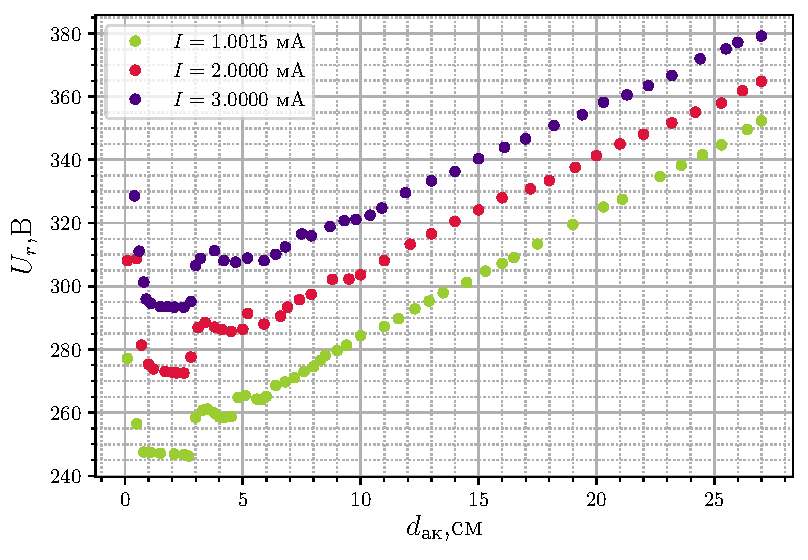
\includegraphics[width=0.75\linewidth]{scripts/fig1}
	\caption{}
	\label{fig:5}
\end{figure}

Область положительного столба начинается там, где зависимость становится 
линейной, а потенциал начинает расти.

Из снятых характеристик определить катодное падение потенциала (полное 
падение потенциала еть сумма катодного потенциала и потенциала в 
положительном столбе):
\begin{gather*}
	I = 1 mA: \Delta U = 261.16-246.27=14.89 \pm 0.02 B \\ 
	I = 2 mA: \Delta U = 288.57-272.53=16.04 \pm 0.02 B \\
	I = 3 mA: \Delta U = 311.24-293.36=17.88 \pm 0.02 B 
\end{gather*}
и продольный градиент потенциала в положительном столбе (от первого 
минимума до первого максимума):
\begin{gather*}
	I = 1 mA: \Delta U = 301.79-297.91=3.88 \pm 0.02 B/cm \\
	I = 2 mA: \Delta U = 320.55-316.56=3.99 \pm 0.02 B/cm \\
	I = 3 mA: \Delta U = 336.33-333.33=3.00 \pm 0.02 B/cm
\end{gather*}

Убедиться, что с ростом силы тока падение потенциала в положительном 
столбе уменьшается. При сближении электродов, катодные части остаются 
без изменения, но положительный столб укорачивается и при неизменной 
силе тока уменьшается напряжение между электродами на величину, равную 
падению напряжения в исчезнувшей части столба.

Найдём на сколько уменьшится напряжение между электродами. Рассмотрим 
расстояние 20 см и 16 см:
\begin{gather*}
	l = 16 cm \\
	I = 1 mA: U = 307.23 B \\
	I = 2 mA: U = 327.97 B \\
	I = 3 mA: U = 342.76 B
\end{gather*}

\begin{gather*}
	l = 20 cm \\
	I = 1 mA: U = 322.24 B \\
	I = 2 mA: U = 341.34 B \\
	I = 3 mA: U = 355.06 B
\end{gather*}

\begin{gather*}
	I = 1 mA: \Delta U = 15.01 B \\
	I = 2 mA: \Delta U = 13.37 B \\
	I = 3 mA: \Delta U = 13.30 B
\end{gather*}

Видно, что при повышении тока, падение потенциала в положительном 
столбе уменьшается.

\subsection{Задание 2}
Вольт-амперная характеристика тлеющего разряда:
\begin{figure}[H]
	\centering
    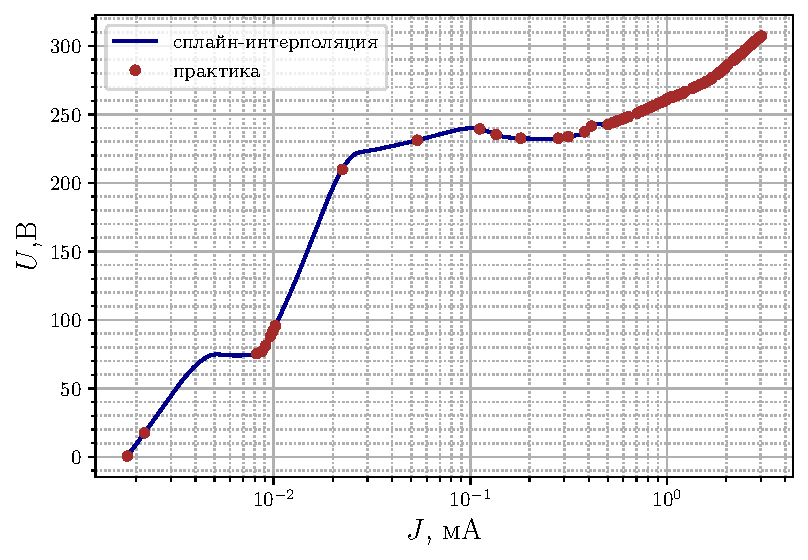
\includegraphics[width=0.75\linewidth]{scripts/fig2}
	\caption{}
	\label{fig:6}
\end{figure}

Для наглядности и для того, чтобы в графике можно было <<узнать>> кривую из 
методички, 
ВАХ строилась в логарифмическом масштабе по оси ординат.


\end{document}
